\section{Problema 1: Cruzando el puente}

    El problema plantea una situación donde dos grupos de personas (arqueólogos y caníbales) se encuentran del lado izquierdo de un puente y buscan cruzarlo. Nuestro objetivo es encontrar el tiempo mínimo necesario para que todos los integrantes del grupo lleguen al otro lado, cumpliendo las siguientes restricciones.

            \begin{itemize}
                \item Solo pueden pasar dos personas a la vez.
                \item En cada cruce es necesario contar con la única linterna presente, que comienza del lado izquierdo.
                \item No puede suceder que en algún lado del puente queden más caníbales que arqueólogos, a menos que solo hayan caníbales.
                \item Cada persona puede cruzar el puente a una velocidad particular. Si dos personas cruzan el puente, lo harán a la velocidad del que sea más lento.
            \end{itemize}

        En las siguientes secciones llamaremos $estado$ a la ubicación de: la linterna, cada arqueólogo y cada caníbal respecto del lado inicial.

        Si numeramos a los integrantes de cada grupo desde 1 hasta N o M (según corresponda), podemos representar cada estado como una tupla $(A,C,L)$, donde $A$ y $C$ son dos vectores de tamaño N y M respectivamente que indican, con un bool, si la ubicación del i-ésimo arqueólogo $A_i$ o caníbal $C_i$ es la del lado final y $L$  indica la ubicación de la linterna. Por lo tanto, cuando todas valgan $True$, habremos llegado al lado final (la linterna no puede terminar del lado inicial porque requeriría que alguien la haya llevado en el último cruce). Ademas, por enunciado, un estado válido tendrá que cumplir:
        \\

        $\sum_{i=0}^{N}\beta(A_i) > 0 \Rightarrow \sum_{i=0}^{N}\beta(A_i) \ge \sum_{i=0}^{M}\beta(C_i)  $
        \ \ \
        $\wedge$
        \ \ \
        $\sum_{i=0}^{N}\beta(\neg A_i) > 0 \Rightarrow \sum_{i=0}^{N}\beta(\neg A_i) \ge \sum_{i=0}^{M}\beta(\neg C_i)$
        \\

        Para cada persona $k$, sabemos su tiempo de cruce $V_k$. También sabemos que la demora de llevar el par $\left \langle {X, Y} \right \rangle$, con $\{X,Y\} \subseteq A \cup C$ (no necesariamente diferentes) de un lado a otro corresponde a $Max\{ V_{X}, V_{Y}  \}$ y es, a su vez, la distancia entre dos estados distintos. De este modo, podemos modelar todas las secuencias de viajes posibles como un grafo ponderado con estados como vértices y donde cada arista es un viaje con peso equivalente a la distancia entre sus vértices adyacentes. De este grafo, finalmente, buscamos la distancia mínima de todos los caminos desde el estado inicial al final que cumplen los requisitos comentados al principio.
        \\
        
\begin{figure}[H]
    \centering
    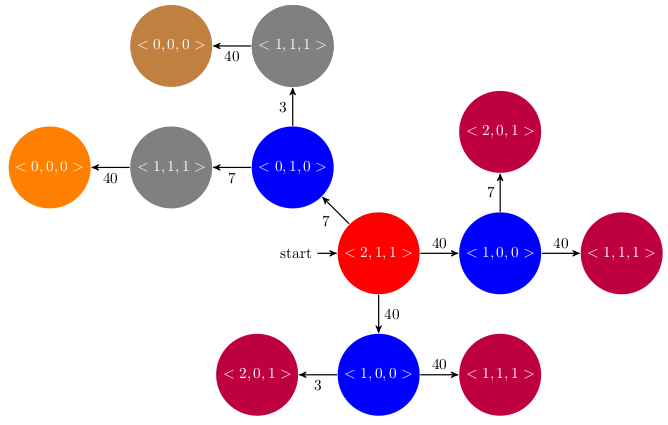
\includegraphics[width=10.0cm]{grafo-ej1}
    \caption{Grafo de estados correspondiente a un ejemplo con dos arqueólogos con valores de demora \{3,7\} y un caníbal con demora de 40. No se presentan todos los estados posibles y solo se indica la cantidad de cada grupo del lado derecho por cuestiones de espacio. La primer componente de cada estado determina la cantidad de arqueólogos del lado inicial, la segunda la cantidad de caníbales y la tercera la linterna. Demora mínima: 50.}
    \label{fig:ej1-graph}
\end{figure}


\subsection{Solución y Correctitud}
    \subsubsection{Solución}

    Para resolver el problema, utilizamos una mecánica basada en el algoritmo de Dijkstra para encontrar caminos mínimos en grafos. La idea es recorrer el grafo empezando desde el estado inicial, conservando el invariante de que conocemos la distancia mínima desde el inicio hasta todos los nodos ya visitados.

    Para ello mantenemos un $map\langle {estado,\ distancia} \rangle$ donde almacenamos los estados ya visitados o candidatos a visitar y su mejor distancia conocida desde el inicio, y un $set$ de tuplas $(distancia, estado)$ ordenado por distancia donde almacenamos los posibles candidatos para el siguiente paso de nuestro recorrido, los vecinos al subgrafo de nodos visitados, y la mejor distancia conocida.

    Recorremos el grafo seleccionando siempre de entre nuestros candidatos el que menor distancia conocida tenga. Como todas las aristas tienen peso positivo, cualquier otro camino que descubramos mas tarde hasta el nodo tendrá una distancia mayor, por lo que podemos asegurar que ya encontramos la mínima. Para cada estado que visitamos debemos corroborar que sea válido, ignorándolo si no cumple las propiedades detalladas anteriormente. Si por lo contrario es un estado válido podemos agregar a la lista de candidatos todos sus vecinos para los cuales la distancia resultante de agregar la arista incidente al camino mínimo que llega al nodo actual es menor a la mejor distancia conocida, reemplazando su entrada como candidato si ya existiera una.

    Si en algún momento visitamos el nodo final, ya sabemos la distancia mínima hasta este por nuestro invariante y podemos detener la búsqueda. Si por otro lado nos quedamos sin candidatos antes de llegar al nodo final podemos asegurar que no existe un camino hasta este, y por lo tanto no existe solución.
\\

\begin{lstlisting}
def TiempoMinimo (velocidadArqueologos : vector<int>, velocidadCanibales : vector<int>)
    map<estado,int> $menorDistancia$
    set<(distancia,estado)> $candidatos$
    marcar la $menorDistancia$ al estado inicial como 0
    agregar el estado inicial a $candidatos$

    while quedan candidatos:
        ($dist$,$actual$) $\leftarrow$ min($candidatos$)
        borrar ($dist$,$actual$) de $candidatos$
        if $actual$ es el estado final: return $dist$

        contar cantidad de arqueologos y canibales de cada lado
        if hay mas canibales que arqueologos de un lado: continue // es un estado invalido

        $estadoHijo$ $\leftarrow$ $actual$
        cambiar el lado de la linterna en $estadoHijo$

        for $x,y \in Arqueologos \times Canibales$: // Pueden ser el mismo
            if $x$ o $y$ no esta del lado de la linterna:
                continue
            cambiar el lado de $x$ e $y$ en $estadoHijo$

            $distanciaCantidato \gets$ max(velocidad de $x$, velocidad de $y$)

            if $estadoHijo$ tiene $menorDistancia$ and $menorDistancia$[$estadoHijo$] $>$ $distanciaCandidato$:
                borrar ($menorDistancia$[$estadoHijo$], $estadoHijo$) de $candidatos$
                borrar $estadoHijo$ de $menorDistancia$

            if $estadoHijo$ no tiene $menorDistancia$:
                $menorDistancia$[$estadoHijo$] $\gets$ $distanciaCandidato$
                agregar ($distanciaCandidato$, $estadoHijo$) a $candidatos$

            reestablecer el lado de $x$ e $y$ en $estadoHijo$ al de $estado$

    return -1 // no hay solucion

\end{lstlisting}

    \subsubsection{Correctitud}

    Usando el modelado del problema sobre el grafo propuesto anteriormente podemos ver que nuestro algoritmo resuelve efectivamente el problema que queríamos resolver. Para esto queremos ver que un camino (sucesión de cambio de estados) mínimo en el problema se traduce en un camino mínimo en el grafo.
    \\

    Para ello necesitamos probar que para todo estado $(A_i,C_j,L_k)$ posible existe un camino simple de distancia $n$ desde el estado de inicio $(A_0,C_0,L_0)$ si y sólo si existe un camino de distancia $n$ entre el vértice $(A_0,C_0,L_0) \rangle$ y el vértice $(A_i, C_j, L_k)$ que recorre vértices asociados a las mismas ubicaciones (todas distintas) en el mismo orden.
    \\

    Esto se ve directamente, ya que por nuestra representación se puede pasar de un estado a otro en tiempo $t$ sii existe una arista en el grafo de peso $t$ entre los nodos que representan a cada estado. Por lo tanto si encontramos un camino mínimo en el grafo vamos a encontrar un camino en el problema, y si existiera una solución mejor al problema entonces existiría un camino del mismo peso en el grafo, y nuestro camino \textit{mínimo} no sería mínimo.
    \\

Veamos que el algoritmo es correcto. Vamos a probar que obtiene siempre la distancia mínima a cualquier vértice del grafo. De ser así, podemos asegurar que el menor camino encontrado para el estado final en particular es efectivamente el mínimo.
\\

Vamos a usar inducción en la cantidad de vértices (estados) visitados en el grafo.
Sea $dist(v)$ la distancia desde el estado inicial obtenida por el algoritmo hasta el vértice $v$. Sea $\delta(v)$, el peso del camino mínimo hasta $v$ y sea $V$ el conjunto de vértices visitados hasta el momento: tenemos que probar que $dist(v) = \delta(v)$ para todo vértice del grafo. Vamos a probarlo mediante inducción con el siguiente lema:
\\

% Estoy martillando esta dem
% https://web.engr.oregonstate.edu/~glencora/wiki/uploads/dijkstra-proof.pdf

\begin{center}
\textbf{Lema: } $\forall$ $v \in$ $V$, $dist(v) = \delta(v)$
\end{center}

\emph{\textbf{Caso Base: }}  Un único vértice visitado. El único momento donde tenemos un solo nodo visitado es al comienzo, es decir
el estado inicial, el cual tiene distancia 0 (por definición) y es correcto trivialmente.
\\

\emph{\textbf{Hipótesis inductiva: }} Para todo vértice explorado anteriormente (es decir que está en $V$) nuestra distancia hallada es la mínima.
\\

\emph{Paso Inductivo:} Sea $u$ el último nodo agregado a $V$. Sea $V'= V + u$, necesitamos probar que $dist(u) = \delta(u)$ para terminar. Vamos por el absurdo, supongamos que nuestro algoritmo no encuentra el camino mínimo: Supongamos que hay un camino más corto hasta $u$ que es $Q$, por lo tanto afirmamos sobre la longitud del camino $Q$, $L(Q)$, que
\\
\begin{center}
\textbf{I)} $L(Q) < dist(u)$
\\
\end{center}
Como $Q$ parte del estado inicial, que llamaremos $S$, y $S \in V$, entonces sabemos que $Q$ empieza en $V$ y en algún momento sale de $V$ para llegar a $u$. Sea $xy$ la primer arista donde $Q$ sale de $V$. Sea $Q_x$ el subcamino de $Q$ con todos sus vértices en $V$, es decir, el subcamino de $Q$ desde $s$ a $x$. Entonces:
\\
\begin{center}
$L(Q_x)+L(xy) \leq L(Q)$
\\
\end{center}
Aplicando H.I, $dist(x)$ es la distancia mínima desde $S$ hasta $x$: $dist(x) \leq L(Q_x)$ y por lo tanto, usando la desigualdad anterior:
\\
\begin{center}
\textbf{II)} $dist(x)+L(xy) \leq L(Q) $
\\
\end{center}
Como $y$ es vecino del vértice (ya visitado) $x$, ya llamamos a $agregarCandidato$ para $y$ iterando sobre $x$. Por lo tanto, o el camino mínimo que tenemos calculado para $y$ es el mínimo para $x$ seguido de la arista que va de $x$ a $y$, o encontramos en algún momento uno mejor. Por lo que vale:
\\
\begin{center}
\textbf{III)} $dist(y) \leq dist(x) + L(xy)$
\\
\end{center}
Por último, como $u$ fue el primer elemento sacado de la cola de prioridad que no pertenece a $V$, tiene menor o igual distancia al estado inicial que el resto de todos los que no pertenecen tampoco a $V$:
\\
\begin{center}
\textbf{IV)} $dist(u) \le dist(y) $
\\
\end{center}
Combinando II) con I) tenemos:
\\
\begin{center}
$dist(x)+L(xy) < dist(u)$
\\
\end{center}
Usando IV) y III) llegamos a:
\\

\begin{center}
    $dist(x)+L(xy) < dist(u) \leq dist(x) + L(xy)$
\\
\end{center}
\textbf{Absurdo}, entonces $Q$ no puede existir siendo menor a la distancia calculada para $u$ y por lo tanto $dist(u) = \delta(u) \QEDB$
\\

Por este mismo absurdo también se puede ver por qué la distancia calculada para cualquier vértice al momento de ser desencolado es, necesariamente, su distancia mínima. Al igual que en la demostración, si existiera otro camino más corto donde alguno de sus vértices todavía no fuera visitado, entonces este vértice no podría estar detrás del estado actual (que viene por un camino distinto) en la cola de prioridad. Como este camino alternativo tendría todavía que llegar al estado final, tiene que sumar \textbf{al menos} una arista más, y como este peso es necesariamente positivo entonces la distancia total no puede ser nunca menor que el tope de la cola de prioridad que se corresponde con la distancia mínima calculada para el próximo estado actual. Partiendo de esto, como guardamos para cada vértice visitado su distancia mínima y solamente encolamos en $agregarCandidato$ cuando la nueva distancia de un hijo es menor que la calculada anteriormente, tenemos asegurado que tampoco vamos a pasar por un estado una vez que este fuera visitado con su mínima distancia.

\subsection{Complejidad}
Antes de empezar a iterar tenemos que inicializar los dos vectores de booleanos que determinan posiciones de arqueólogos y caníbales, y agregar el estado inicial como candidato. Esto nos cuesta $\mathcal{O}(N+M)$. \\

El peor caso teórico sería aquel en el que tuviéramos que visitar todos los estados configurables del grafo (asumiendo que todos fueran posibles y no fueran podados) y tener que encolar/actualizar todas las distancias por cada estado generado por cada par posible.

La cantidad de estados totales que tendremos será $2^{N+M+1}$ porque por cada arqueólogo, caníbal y linterna pueden o ser $True$ o $False$. \\

El costo de actualizar una distancia, asumiendo que todos los estados están presentes en el diccionario y en el conjunto que usamos como cola de prioridad, es logarítmico en su cantidad de elementos\footnote{The C++ standard (n4296), \textsection 23.4.4}: $\mathcal{O}(log(2^{N+M}) * cmp(estado) + copy(estado)) = \mathcal{O}((N+M) * cmp(estado) + N+M) = \mathcal{O}((N+M) * (N+M) + N+M) = \mathcal{O}((N+M)^2)$. \\

La cantidad de pares de elementos de $A$ es cuadrática en sus elementos (contando la posibilidad de elegir dos veces al mismo, siendo un único elemento que cambie entre estados), ídem para $C$ y para pares mixtos hay $M*N$ combinaciones.

Por lo tanto tenemos un costo de $\mathcal{O}((N^2+M^2+N*M)*(N+M)^2) = \mathcal{O}(N^4+M^4)$ para actualizar todos los estados $hijos$ posibles del estado actual. \\

Luego, en cada iteración desencolamos un estado nuevo estado y lo eliminamos del árbol. Por lo que dijimos antes respecto de los árboles, esto tiene un costo de orden $\mathcal{O}((N+M)^2)$. \\

Juntando todo nos queda una complejidad de $\mathcal{O}(Inicializar\ vectores\ +\ Cantidad\ de\ estados*(Desencolar\ nuevo\ estado\ + Insertar\ hijos)) = \mathcal{O}((N+M)^2+2^{N+M}((N+M)^2+(N^4+M^4))) = \mathcal{O}(\ 2^{N+M}*(N^4+M^4)\ )$

\subsection{Análisis experimental}

En la anterior sección teorizamos un peor caso que forzaba a visitar y procesar cada estado que fuera posible dentro del grafo suponiendo que además también forzaría a actualizar, para las dos estructuras, todos los hijos de estos estados en cada iteración. Intentando buscar alguna manera de arreglar las velocidades de cada vector para generar condiciones similares (como por ejemplo, que el último estado en visitarse sea el final) nos encontramos con que no es trivial encontrar semejantes disposiciones. Aún así, apelando a ese análisis de complejidad, podemos aprovechar que no influye en la complejidad final el valor de las velocidades (en tanto se generen estos peores casos) y termina siendo en función de los tamaños de los vectores. Por lo tanto generamos casos de test sobre combinaciones de tamaños para ambos vectores y eligiendo velocidades uniformemente entre $1$ y $10^6$.
\\

\begin{figure}[H]
    \centering
    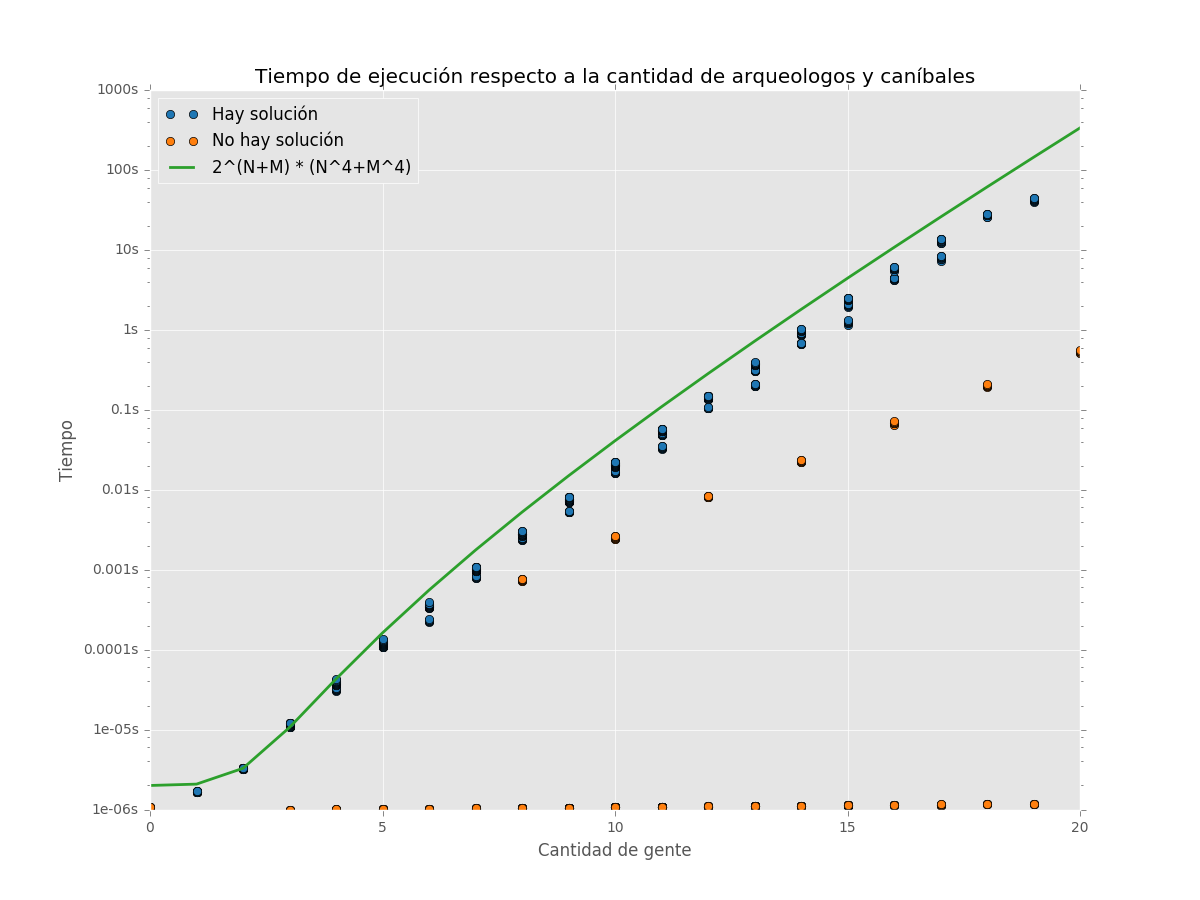
\includegraphics[width=\textwidth]{ej1}
    \caption{Tiempo de ejecución en función de la suma de cantidad de arqueólogos y cantidad de caníbales. Las velocidades de cada uno son generadas a partir de una distribución uniforme entre $1$ y $10^6$. Cada medición es el tiempo mínimo de 10 corridas.}
    \label{fig:ej1-fig}
\end{figure}

Las muestras de la figura \ref{fig:ej1-fig} se toman a partir de todas las combinaciones posibles de entre 0 y 10 elementos por cada vector, con al menos 2 repeticiones por caso. Es por esto que se pueden ver 'outliers' de muy bajo tiempo de ejecución, que se corresponden a los casos donde la cantidad de caníbales es mayor a la de arqueólogos y por lo tanto la poda de estados que no cumplan las condiciones de mayoría de arqueólogos por cada lado acaba por recortar todos los candidatos en las primeras iteraciones. 

Recordando que en la sección previa llegamos a una complejidad de orden $ \mathcal{O}(\ 2^{N+M}*(N^4+M^4)\ )$ y consideramos un eje de coordenadas $x = M + N$, sería acorde que si la cota estuviera bien ajustada pudiéramos observar para cada combinación de tamaños de valor $x$ un tiempo de ejecución resultante de orden $ 2^{x} x^4 $. Esto se condice con nuestras muestras.

